\documentclass{beamer}
\usetheme{Madrid}

 \pdfmapfile{+sansmathaccent.map}

\renewcommand{\familydefault}{\rmdefault}

\usepackage{amsmath}
\usepackage{mathtools}

\DeclareMathOperator*{\argmin}{arg\,min}

\title{Discrete Systems}
\author{by Sergei Savin}
\centering
\date{Spring 2020}

\begin{document}
\maketitle


\begin{frame}{Content}
\begin{itemize}
\item Discretization
\item ZOH and Precise discretization
\item Stability
\end{itemize}
\end{frame}

\begin{frame}{Discretization}
\framesubtitle{Finite difference}
\begin{flushleft}

Consider linear time-invariant autonomous system:

\[
\dot {\mathbf x} = \mathbf A \mathbf x
\]

The time derivative $\dot {\mathbf x}$ can be replaces with a finite difference:

\[
\dot {\mathbf x} \approx \frac{1}{\Delta t}(\mathbf x(t + \Delta t) - \mathbf x(t))
\]

Note that we could have also used other definitions of a finite difference:

\[
\dot {\mathbf x} \approx \frac{1}{\Delta t}(\mathbf x(t + 0.5\Delta t) - \mathbf x(t - 0.5\Delta t))
\]

or

\[
\dot {\mathbf x} \approx \frac{1}{\Delta t}(\mathbf x(t) - \mathbf x(t - \Delta t))
\]

\end{flushleft}
\end{frame}

\begin{frame}{Discretization}
\framesubtitle{Finite difference notation}
\begin{flushleft}
We can introduce notation:

\[
\begin{cases}
\mathbf x[0] = \mathbf x(0) \\
\mathbf x[1] = \mathbf x(\Delta t) \\
\mathbf x[2] = \mathbf x(2\Delta t) \\
... \\
\mathbf x[n] = \mathbf x(n\Delta t) 
\end{cases}
\]

We say that $ x[i]$ is the value of $x$ at the time step $i$. Then the finite difference can be written, for example, as follows:

\[
\dot {\mathbf x} \approx \frac{1}{\Delta t}(\mathbf x[i + 1] - \mathbf x[i])
\]

\end{flushleft}
\end{frame}



\begin{frame}{Discretization}
\framesubtitle{Finite difference in an autonomous LTI}
\begin{flushleft}

We can rewrite our original autonomous LTI as follows:

\[
\frac{1}{\Delta t}(\mathbf x[i + 1] - \mathbf x[i]) = \mathbf A \mathbf x[i]
\]
Isolating $\mathbf x[i + 1]$ on the left hand side, we get:
\[
\mathbf x[i + 1] = (\mathbf A \Delta t + \mathbf I) \mathbf x[i]
\]

\noindent\rule{12cm}{0.4pt}

Or alternatively:

\[
\frac{1}{\Delta t}(\mathbf x[i + 1] - \mathbf x[i]) = \mathbf A \mathbf x[i + 1]
\]
Isolating $\mathbf x[i + 1]$ on the left hand side, we get:
\[
\mathbf x[i + 1] = (\mathbf I - \mathbf A \Delta t)^{-1} \mathbf x[i] 
\]

\end{flushleft}
\end{frame}

\begin{frame}{Discretization}
\framesubtitle{Discrete LTI, part 1}
\begin{flushleft}

If we have dynamics in the form:
\[
\dot {\mathbf x} = \mathbf A \mathbf x + \mathbf B \mathbf u
\]
%
we can do the same transformation as before:
\[
\frac{1}{\Delta t}(\mathbf x[i + 1] - \mathbf x[i]) = \mathbf A \mathbf x[i] + \mathbf B \mathbf u[i]
\]
\[
\mathbf x[i + 1] = (\mathbf A \Delta t + \mathbf I) \mathbf x[i] + \mathbf B \Delta t \mathbf u[i]
\]

\end{flushleft}
\end{frame}


\begin{frame}{Discretization}
\framesubtitle{Zero order hold}
\begin{flushleft}

Defining \emph{discrete state space matrix} $\bar{\mathbf A}$ and \emph{discrete control matrix} $\bar{\mathbf B}$ as follows:

\[
\bar{\mathbf A} = (\mathbf A \Delta t + \mathbf I),\;  \bar{\mathbf B} = \mathbf B \Delta t
\]
%
We get discrete dynamics:

\[
\mathbf x[i + 1] = \bar{\mathbf A} \mathbf x[i] + \bar{\mathbf B} \mathbf u[i]
\]

This way of defining discrete dynamics is called \emph{Zero order hold}.

\end{flushleft}
\end{frame}


\begin{frame}{ZOH and other types of discretization}
\framesubtitle{Zero order hold vs First order hold}
\begin{flushleft}

Graphically, we can understand what zero order hold is, by comparing it to the first order hold:

\begin{figure} [h!]
\begin{center}
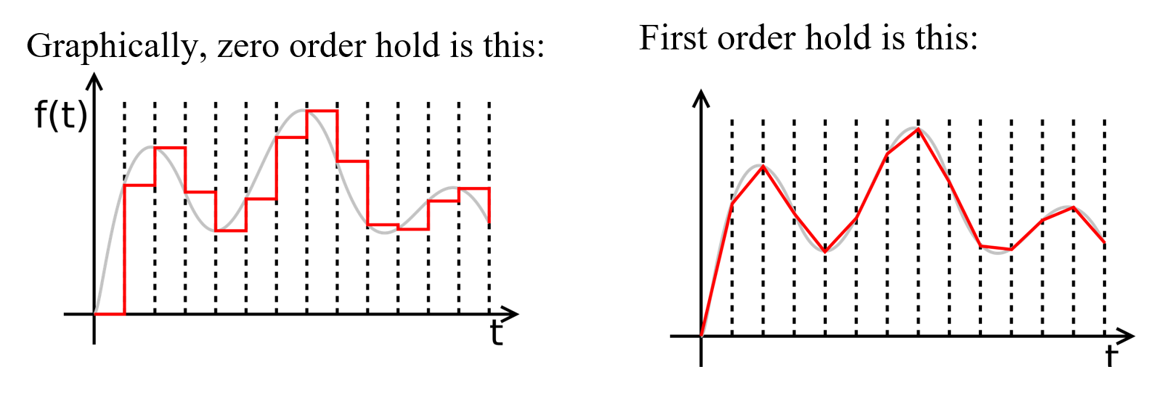
\includegraphics[width=3.5in]{ZOH.PNG}
\end{center} 
\caption{Different types of discretization} \label{F:ZOH}
\end{figure}

\end{flushleft}
\end{frame}


\begin{frame}{ZOH and other types of discretization}
\framesubtitle{Precise discretization}
\begin{flushleft}

Let the discrete state $\mathbf x[i]$ correspond to the moment of time continuous state $\mathbf x$ at the moment of time $t_i$, and $\mathbf x[i + 1]$ - to the point of time $t_{i+1}$. Then, we can say that the discretization is \emph{exact} if there is the following implication relation

\[
\mathbf x[i] = \mathbf x(t_i) \rightarrow 
\mathbf x[i+1] = \mathbf x(t_{i+1})
\]
%
or in other words, if state of both systems are identical for the discrete time points where the discrete states are defined. 

We can compute exact discretization as follows:

\[
\bar{\mathbf A} = e^{\mathbf A \Delta t}
\]
\[
\bar{\mathbf B} = \mathbf B \int_{t_0}^{t_0 + \Delta t} e^{\mathbf A s} ds
\]


\end{flushleft}
\end{frame}

\begin{frame}{Stability criterion}
\begin{flushleft}

For continuous-time systems $\dot {\mathbf x} = \mathbf A \mathbf x$, the criterion is that the real parts of the eigenvalues of the matrix $\mathbf A$ are all negative.

\bigskip

For a discrete time system $\mathbf x[i + 1] = \bar{\mathbf A} \mathbf x[i]$, the criterion for the stability in the sense of Lyapunov is that all eigenvalues should be less than 1 by magnitude:

\[
|\lambda_i(\bar{\mathbf A})| \leq 1, \; \forall i
\]

if $|\lambda_i(\bar{\mathbf A})| < 1, \; \forall i$, the system is asymptotically stable (or just stable).

\end{flushleft}
\end{frame}



\begin{frame}
\centerline{Lecture slides are available via Moodle.}
\bigskip
\centerline{Check Moodle for additional links, videos, textbook suggestions.}
\end{frame}

\end{document}
